\documentclass{article}
\usepackage{iclr2026_conference,times}
\input{math_commands.tex}
\usepackage{hyperref}
\usepackage{url}
\usepackage{graphicx}
\usepackage{booktabs}
\usepackage{multirow}
\usepackage{amsmath}
\usepackage{xcolor}

\title{ProjectEgo: An Evidence-Backed Observatory and Utility Benchmark\\for Egocentric Data in Robot Learning}

% Keep the submission anonymous. Uncomment \iclrfinalcopy and replace this block
% only after acceptance or when producing a clearly labeled non-anonymous draft.
\author{Anonymous authors}

% \iclrfinalcopy
\begin{document}
\maketitle

\begin{abstract}
Egocentric datasets are increasingly used to pretrain embodied models and to transfer human experience to robots, yet their descriptions are fragmented across vision, wearable sensing, and robotics. Scale and modality lists are frequently treated as proxies for quality even when releases differ in viewpoint, action observability, licensing, and evidence. We introduce ProjectEgo, a living dataset observatory and reproducible benchmark that separates reported metadata, measured data quality, and downstream robot utility. ProjectEgo represents versioned releases along a continuum from human first-person observation to robot-native trajectories, attaches field-level provenance and evidence levels to every claim, and evaluates six quality dimensions without collapsing task-dependent trade-offs into a universal ranking. The current reproducible snapshot tracks 109 candidates and contains 20 cross-checked anchor releases spanning 2011--2026 and 15 modality signals. We further formalize the Ego-to-Robot Gap and specify fixed-budget transfer experiments for measuring dataset utility. This paper presents the taxonomy, evidence model, audit protocol, and benchmark design; file-level audits and controlled policy experiments are explicitly identified as the remaining requirements for a complete benchmark claim.
\end{abstract}

\section{Introduction}

Foundation models have shifted the robotics data problem from collecting demonstrations for one robot and task toward assembling experience broad enough to support transferable perception, reasoning, and behavior. Robot-native trajectories provide executable controls but are expensive and embodiment-specific. Human egocentric data capture natural behavior, dexterous interaction, long-horizon intent, and open-world context at much greater scale, but often omit force, geometry, state, and action signals needed for control.

The resulting question is not simply which dataset is largest, but \emph{which egocentric data, under which evidence and budget, are useful for which robot-learning objective?} Existing first-person vision surveys organize tasks and methods \citep{betancourt2015evolution,bandini2023hands,yao2021future,plizzari2024outlook,li2025challenges}. Dataset pages and catalogs commonly emphasize reported hours and modality checkmarks. Neither view establishes whether files are accessible, internally valid, or useful for a specified robot-learning task.

ProjectEgo addresses this gap through four contributions:
\begin{enumerate}
    \item a scope and taxonomy connecting human ego, paired ego--exo, robot-free, and robot-native data;
    \item a versioned catalog in which material fields are linked to sources, timestamps, and evidence levels;
    \item a multidimensional quality standard that separates observable quality from task-specific utility; and
    \item a benchmark design based on fixed budgets, learning curves, cross-dataset transfer, and uncertainty.
\end{enumerate}

The present release is a methods and infrastructure paper, not a claim that all candidate datasets have been fully audited. It provides a reproducible level-2 cohort of 20 anchor releases and defines the experiments required to reach level 5. This distinction is central: a benchmark should expose what has been measured rather than reward unsupported precision.

\begin{figure}[t]
  \centering
  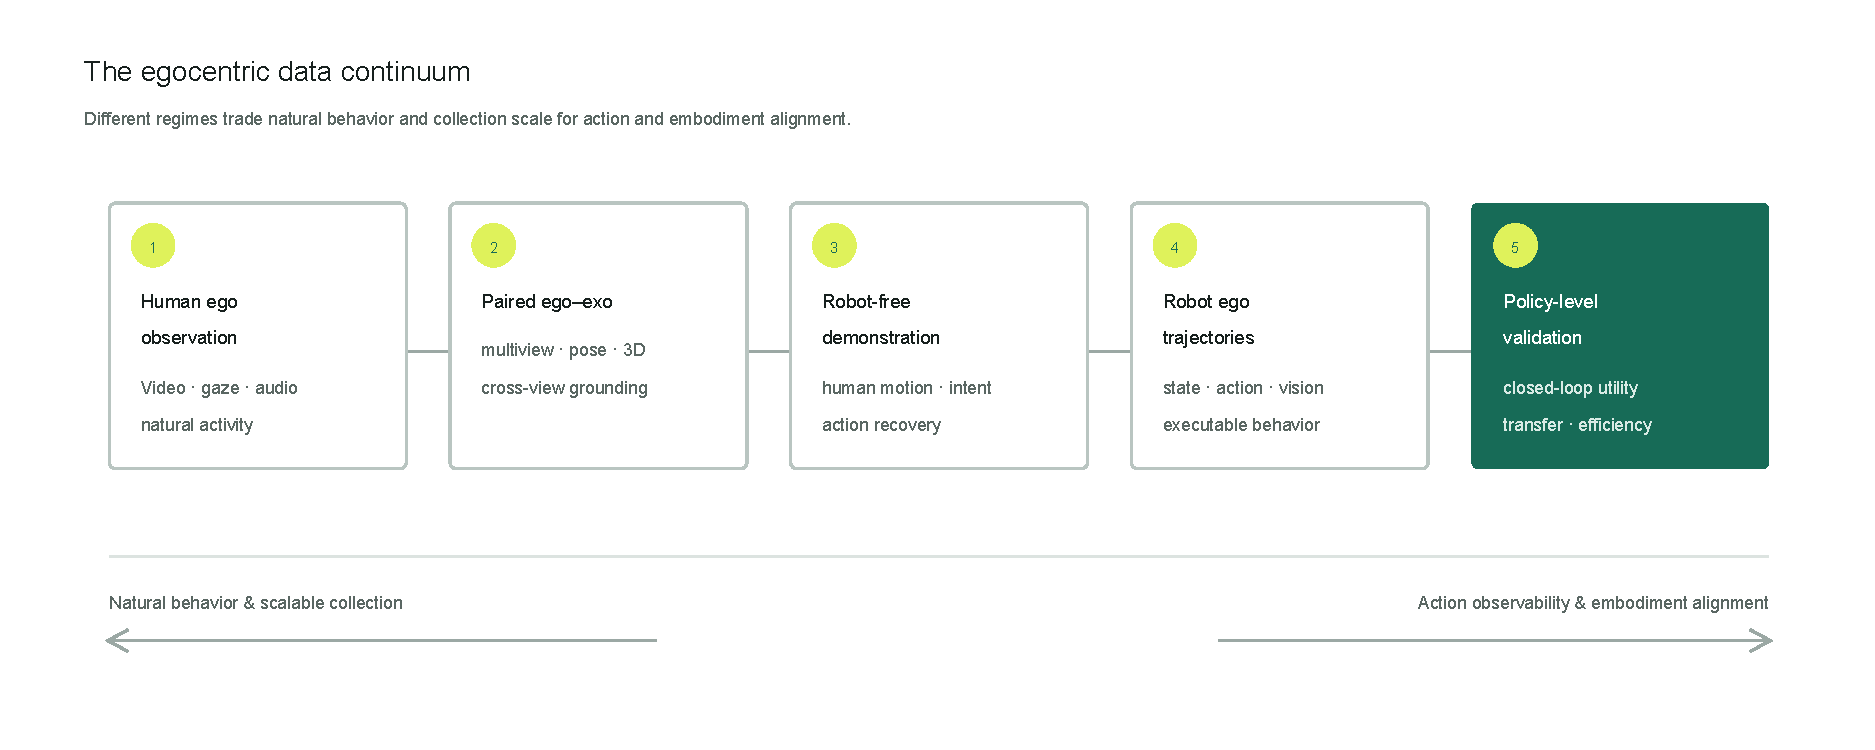
\includegraphics[width=\linewidth]{figures/projectego-scope.pdf}
  \caption{ProjectEgo treats data as a continuum. Moving toward robot-native trajectories generally improves action and embodiment alignment while increasing collection cost. Evidence level is independent of regime.}
  \label{fig:scope}
\end{figure}

\section{Related Work}

\paragraph{Egocentric vision.}
Early surveys established first-person vision as a field spanning activity recognition, object interaction, lifelogging, and assistive systems \citep{betancourt2015evolution}. Later reviews studied hands, anticipation, and always-on perception \citep{bandini2023hands,yao2021future,plizzari2024outlook}. Large datasets progressed from GTEA \citep{fathi2011gtea} and EGTEA Gaze+ \citep{li2018egtea} to EPIC-KITCHENS \citep{damen2022epic}, Ego4D \citep{grauman2022ego4d}, and Ego-Exo4D \citep{grauman2024egoexo}. These resources establish the perceptual side of the landscape but do not by themselves measure robot-policy utility.

\paragraph{Robot-learning data.}
BridgeData V2, Open X-Embodiment, DROID, RH20T, and RoboMIND broaden robot data across environments, institutions, sensors, tasks, and embodiments \citep{walke2023bridge,oxe2024,khazatsky2024droid,fang2024rh20t,wu2025robomind}. Their action-aligned supervision provides an essential reference for evaluating human-to-robot transfer.

\paragraph{Human-to-robot transfer.}
Recent systems increasingly treat wearable human demonstrations as policy data rather than representation data. EgoZero and EgoVerse are representative of this direction \citep{liu2025egozero,punamiya2026egoverse}. Their results motivate controlled cross-dataset evaluation, but headline success rates are not directly comparable when robots, tasks, policies, and budgets differ.

\section{Review and Catalog Protocol}

\subsection{Unit of analysis and eligibility}

The unit is a \emph{versioned dataset release}, not a paper. A family may include an original release, successor, annotation extension, benchmark split, and mirror. These are linked rather than silently collapsed or double-counted. Human first-person, robot-mounted, paired ego--exo, synthetic ego, and dataset mixtures are eligible. Third-person-only data require paired observations or a material ego-transfer contribution. Closed datasets may be cataloged from public evidence, but inaccessible fields cannot receive file-level scores.

The search covers scholarly indexes, major computer-vision and robotics venues, artifact registries, dataset hosts, project pages, challenge sites, citation graphs, and existing curated lists. Exact-name and backward/forward citation searches are performed for included anchors. Candidate discovery does not imply verification.

\subsection{Evidence ladder}

Every material claim is assigned the highest supported evidence level (Table~\ref{tab:evidence}). The ladder prevents two category errors: documentation is not technical validity, and technical validity is not downstream usefulness.

\begin{table}[t]
\caption{ProjectEgo evidence levels. Higher levels require direct inspection or experiments.}
\label{tab:evidence}
\centering
\small
\begin{tabular}{clp{3.3in}}
\toprule
Level & Name & Permitted interpretation \\
\midrule
1 & Claimed & A paper, official page, or maintainer states the claim. \\
2 & Metadata & Structured metadata is cross-checked across two sources. \\
3 & Sampled & The claim holds for a documented sample of released files. \\
4 & Verified & A full applicable automated audit passes within stated limits. \\
5 & Validated & Controlled downstream utility is measured for a task and budget. \\
\bottomrule
\end{tabular}
\end{table}

The current anchor cohort requires a primary paper and a second official or attributed source. Conflicts are retained in notes, unknown values remain missing, and trajectories are never converted to hours using an assumed duration. Release year is stored separately from reference-paper publication year.

\subsection{Reproducible snapshot}

The frozen discovery snapshot contains 109 candidate records. Twenty releases currently satisfy the level-2 anchor rule: eight human-ego, seven paired ego--exo, and five robot-ego records. They span 2011--2026 and 15 controlled modality signals. The machine-readable source, generated master table, statistics, and plotting script are versioned together. Figures~\ref{fig:timeline} and \ref{fig:modalities} describe this selected cohort and are not estimates of field prevalence.

\begin{figure}[t]
  \centering
  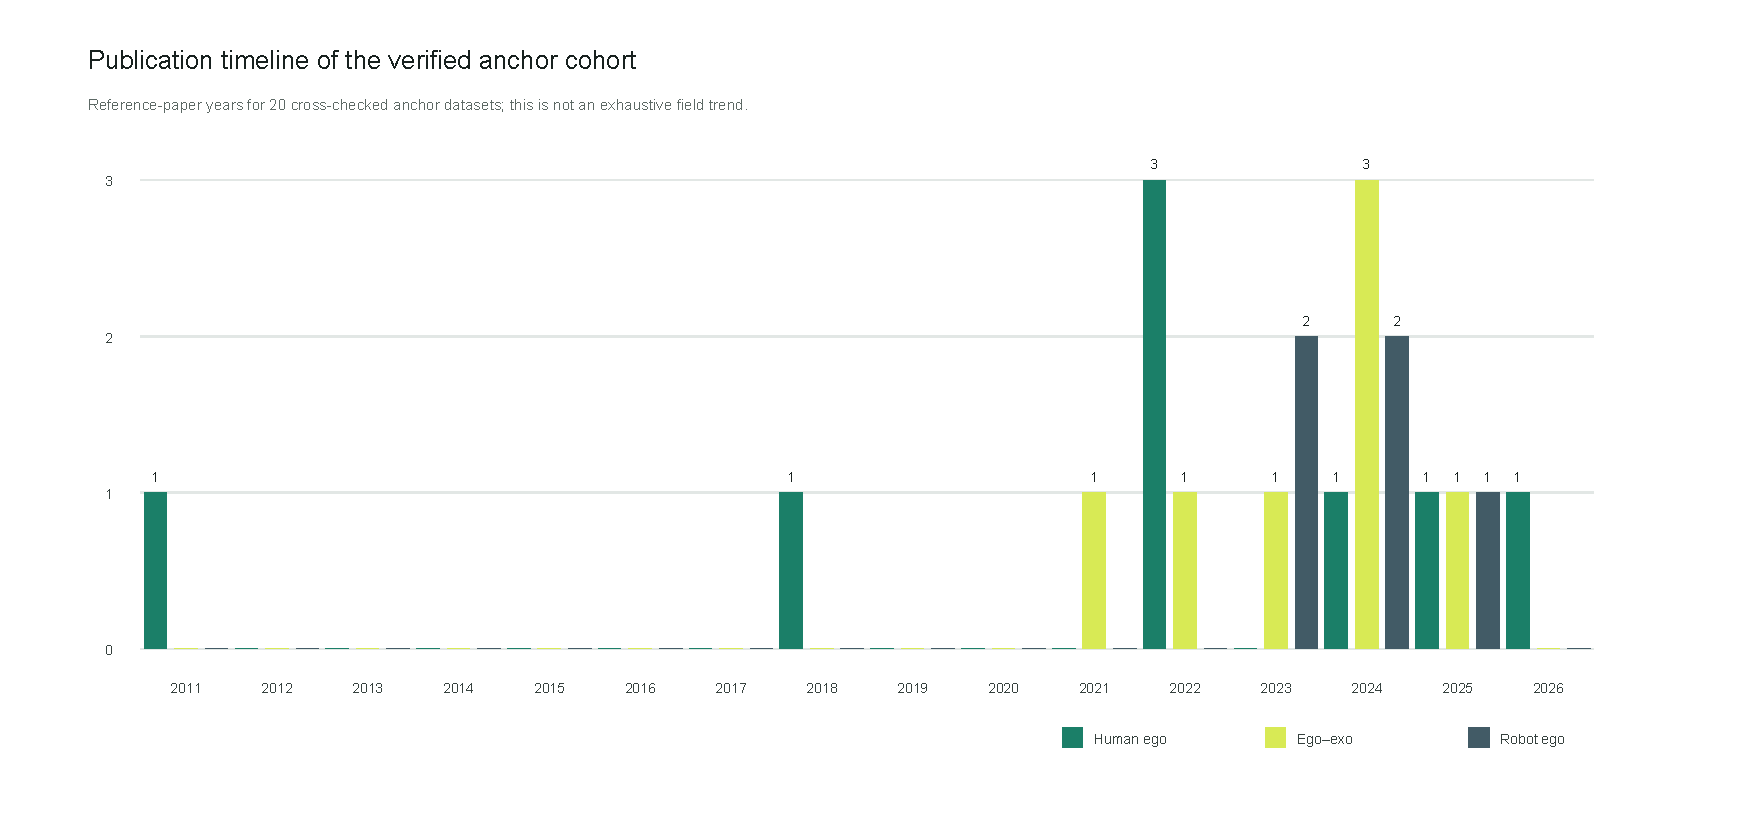
\includegraphics[width=\linewidth]{figures/anchor-release-timeline.pdf}
  \caption{Reference-paper timeline for the 20 level-2 anchors. Empty years are retained. Selection is deliberately bounded and is not an exhaustive historical frequency estimate.}
  \label{fig:timeline}
\end{figure}

\begin{figure}[t]
  \centering
  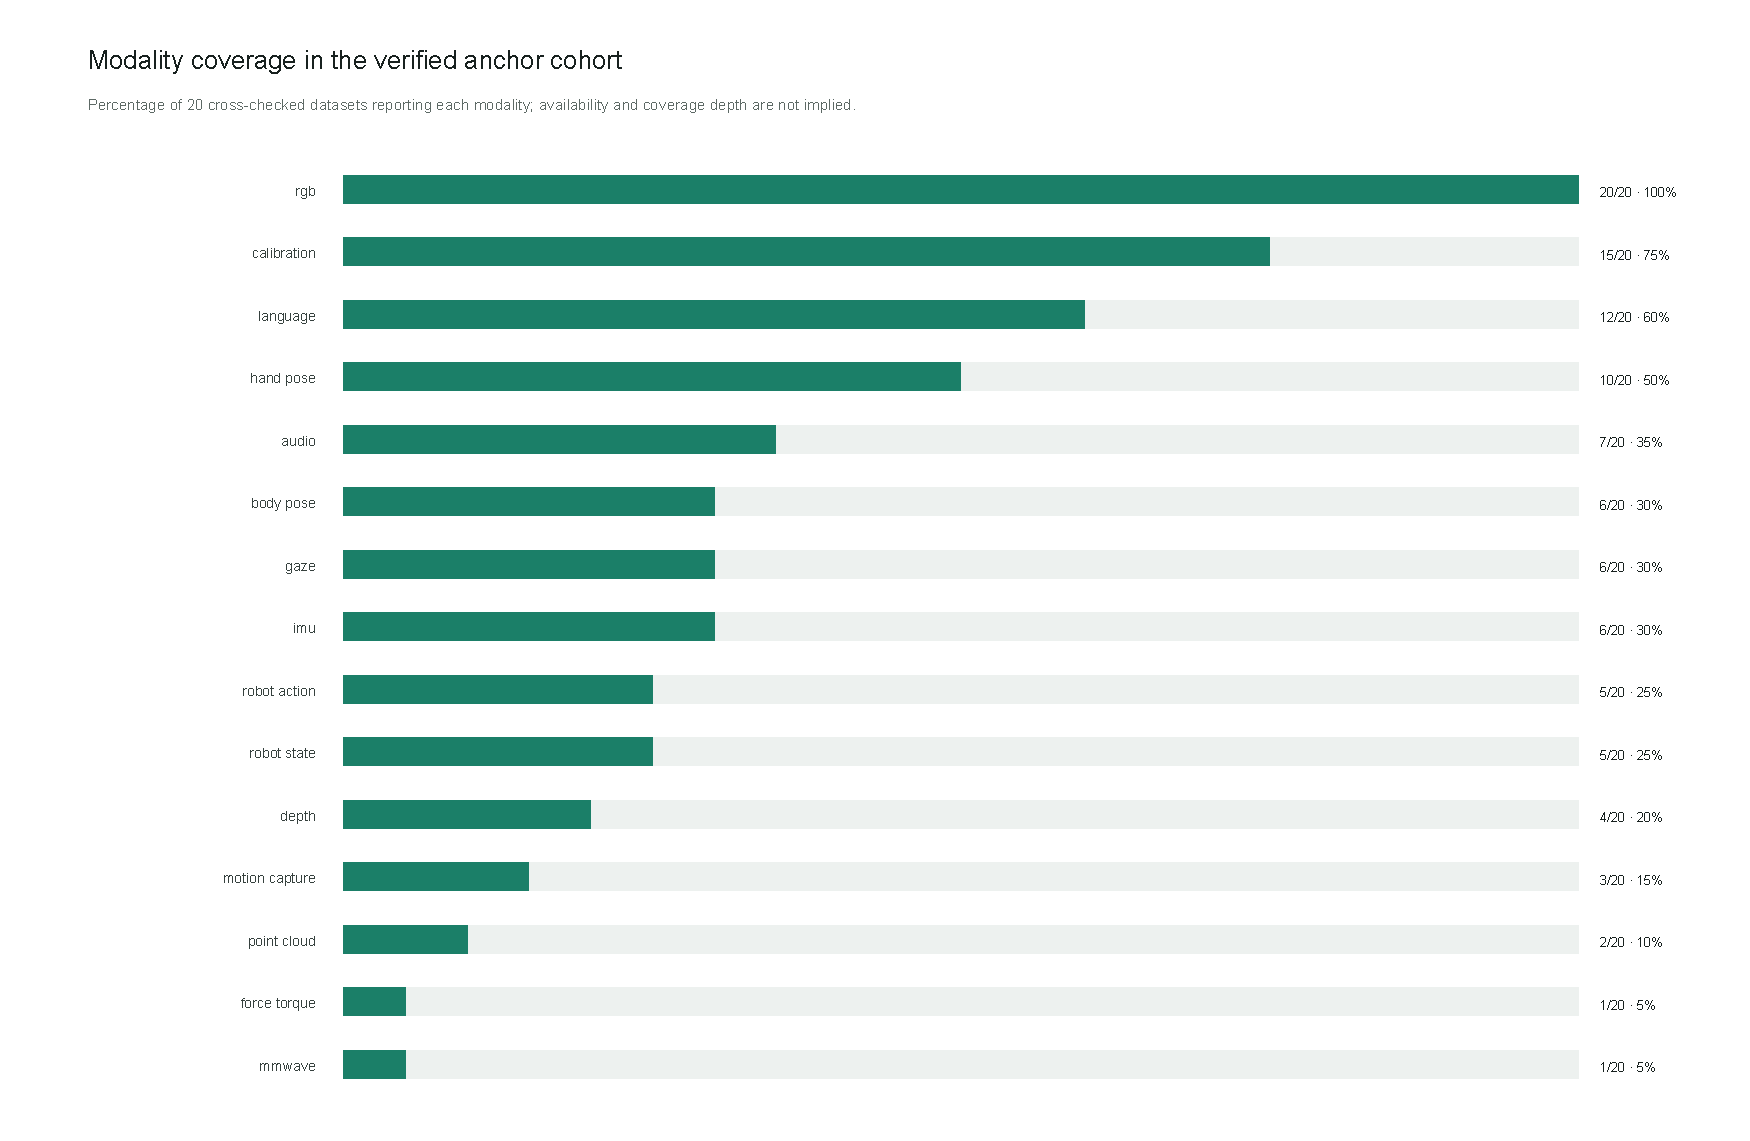
\includegraphics[width=\linewidth]{figures/anchor-modality-coverage.pdf}
  \caption{Reported modality coverage in the anchor cohort. Presence does not imply full-release coverage, file validity, or synchronization quality.}
  \label{fig:modalities}
\end{figure}

\section{A Taxonomy for Egocentric Robot Data}

Viewpoint is necessary but insufficient. ProjectEgo defines egocentric data as observations captured from, attached to, or intentionally approximating the situated viewpoint of an acting human, robot, or embodied agent. Robot-learning relevance arises through perception, temporal and intent modeling, human-motion recovery, world-model pretraining, or policy learning and evaluation.

We encode independent axes rather than a single dataset category: capture agent and embodiment; viewpoint and camera placement; sensing and calibration; supervision and annotations; action observability; environment and population; access, license, and governance; and intended use. This avoids treating a long modality list as a sufficient quality description.

\begin{figure}[t]
  \centering
  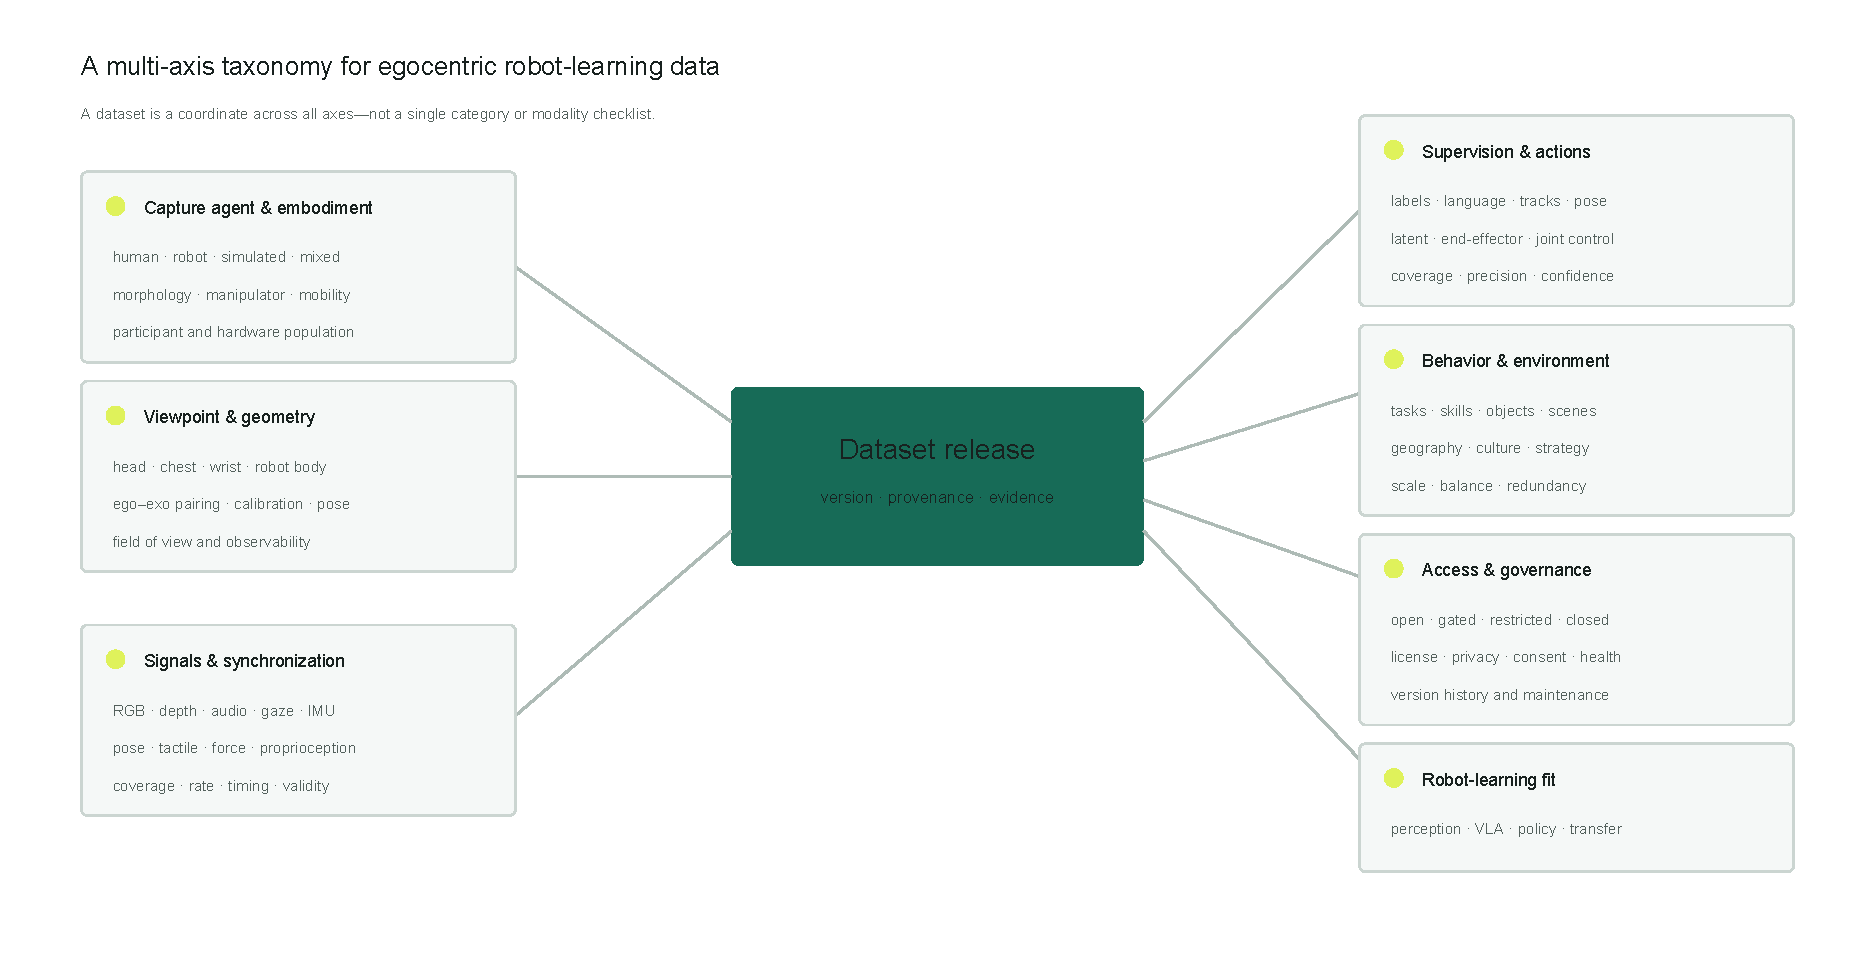
\includegraphics[width=\linewidth]{figures/projectego-taxonomy.pdf}
  \caption{Independent dataset axes used by ProjectEgo. Human-to-robot alignment is represented explicitly rather than inferred from first-person viewpoint.}
  \label{fig:taxonomy}
\end{figure}

The taxonomy supports five non-exclusive regimes. Human egocentric observation maximizes natural behavior but lacks executable action. Paired ego--exo capture improves 3D grounding and reduces occlusion. Robot-free demonstrations add portable tracking or action recovery without occupying a robot. Robot-native trajectories provide direct state-action supervision but introduce platform bias and collection cost. Synthetic or transformed ego data can add controlled variation but must expose generation assumptions and sim-to-real limitations.

\section{Quality Is a Vector, Not a Universal Score}

ProjectEgo evaluates six dimensions: (1) integrity and technical validity; (2) perceptual quality; (3) semantic and annotation quality; (4) diversity, coverage, and scale; (5) access, governance, and reproducibility; and (6) robot-learning utility. Each dimension contains observable tests and evidence coverage. Missing evidence is not converted to zero, because absence of evidence and measured failure have different meanings.

For dimension $d$, let $s_d$ be a normalized score computed only from applicable tests, $c_d$ the evidence coverage, and $u_d$ an uncertainty estimate. We report $(s_d,c_d,u_d)$ rather than one intrinsic rank. Given target task $T$, user constraints $C$, and explicit weights $w_{T,d}$, a recommendation can be computed only after hard constraints such as license and required modalities are applied:
\begin{equation}
S(D\mid T,C)=\sum_{d \in \mathcal{D}_T} w_{T,d}\,s_d\,c_d,
\qquad \sum_d w_{T,d}=1.
\end{equation}
This is a decision score, not a claim of universal dataset quality. Rankings must expose weights, missing fields, evidence levels, and sensitivity to alternative reasonable weights.

\section{The Ego-to-Robot Gap}

Human first-person data and robot trajectories differ along at least six observable axes: viewpoint, embodiment, action representation, dynamics and contact, intent and task specification, and environment distribution. We denote the gap vector
\begin{equation}
\mathbf{g}(H,R)=[g_{view},g_{emb},g_{act},g_{dyn},g_{intent},g_{env}].
\end{equation}
The vector is diagnostic rather than directly additive. A transformation may reduce one component while increasing another; for example, hand-pose retargeting improves action observability but introduces reconstruction and morphology error. Dataset cards should therefore state what alignment signals exist and what transformations are required before policy learning.

\section{Utility Benchmark Design}

Metadata cannot establish utility. ProjectEgo proposes fixed-budget experiments with a shared policy family, controlled compute, frozen evaluation tasks, repeated seeds, and leakage checks. The benchmark separates representation pretraining, action recovery, policy pretraining, and target-task adaptation. For each dataset or mixture, it reports zero-shot performance where meaningful, few-shot adaptation, area under the data-efficiency curve, final success, robustness under viewpoint and environment shifts, and variance.

\begin{figure}[t]
  \centering
  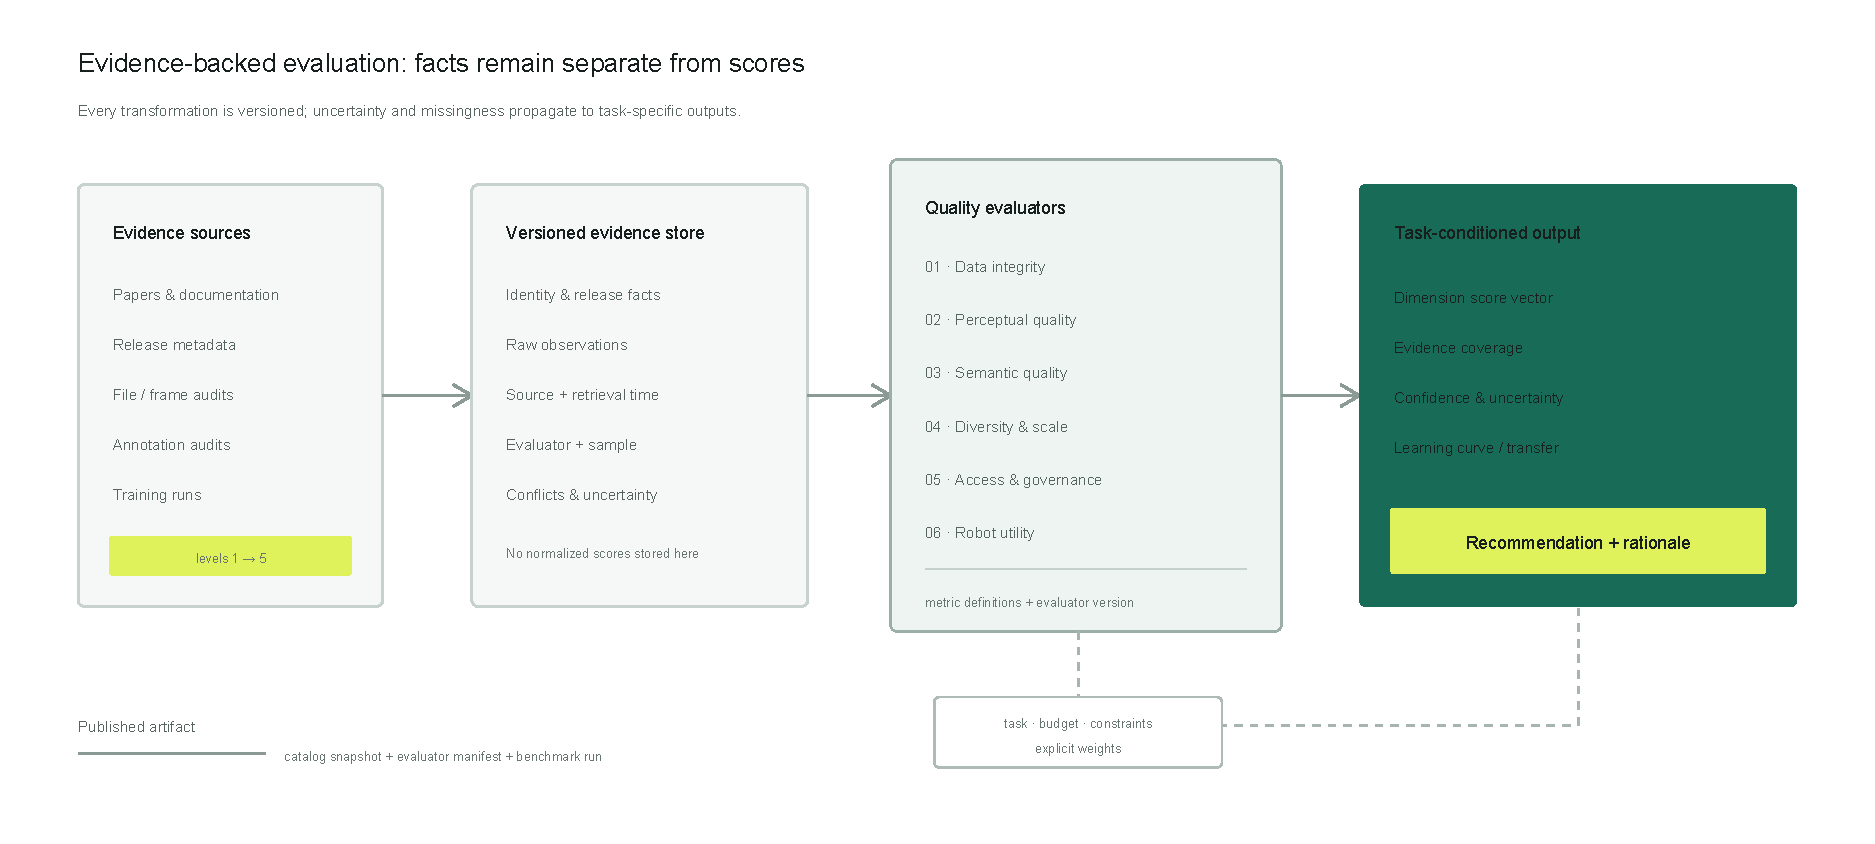
\includegraphics[width=\linewidth]{figures/projectego-evaluation.pdf}
  \caption{Evidence-backed evaluation pipeline. Facts and measurements remain separate from task-weighted recommendation scores.}
  \label{fig:evaluation}
\end{figure}

The first experimental matrix should include at least three task families: language-conditioned tabletop manipulation, dexterous hand--object interaction, and long-horizon mobile manipulation. Each family should compare human ego, paired ego--exo, robot-native, and mixture conditions under equal token/frame and compute budgets. A no-pretraining baseline and a robot-only reference are required. Dataset identity must be isolated from preprocessing differences, and confidence intervals must be reported across tasks and seeds.

\section{Limitations, Ethics, and Reproducibility}

The current 20-record cohort is level 2: it validates the schema and evidence workflow, not the underlying files or downstream utility. It is selected to cover regimes and eras rather than sampled to estimate prevalence. Hours can be incomparable across unique wall-clock activity, synchronized multi-view video, and robot operating time. Licenses and access conditions can change after a snapshot.

Egocentric capture raises privacy risks involving homes, screens, conversations, and bystanders. Redaction may remove learning signals, and consent may be difficult to maintain in long-duration recording. A quality benchmark must record governance evidence and avoid rewarding scale acquired through weak consent or unclear redistribution rights.

The catalog source, generated outputs, protocol, and figure builder are versioned. Reproduction requires rebuilding derived files from the frozen JSON cohort and checking that no generated diff appears. Future releases will add field-level provenance objects, independent dual extraction, sampled file manifests, and benchmark containers.

\section{Conclusion}

Egocentric data cannot be ranked responsibly by scale or modality count alone. ProjectEgo reframes dataset selection as an evidence-backed decision problem connecting human observation to robot utility. The current release contributes a taxonomy, evidence ladder, reproducible 20-anchor catalog, and controlled benchmark design. The decisive next step is empirical: file-level audits and fixed-budget transfer experiments must demonstrate which datasets help which robots learn.

\bibliography{references}
\bibliographystyle{iclr2026_conference}

\appendix
\section{Planned audit modules}

The level-3/4 audit suite will include archive and checksum verification; decode success and temporal continuity; missing and duplicate frame detection; timestamp monotonicity; sensor synchronization; calibration residuals; annotation schema and boundary checks; split leakage; access and license snapshots; and coverage estimates with confidence intervals. Every module will emit machine-readable observations, tool versions, sampled paths, and failure examples.

\section{Planned benchmark reporting}

Every utility result will identify dataset release, preprocessing commit, policy and optimizer, trainable parameter count, token/frame budget, compute budget, target tasks, seeds, evaluation episodes, confidence interval, and failure taxonomy. Results without sufficient artifact access will remain unscored rather than assigned a penalty that conflates access with measured quality.

\section{Submission-status disclosure}

This source is an ICLR-format research draft. The current public release supports metadata-level claims only. Statements describing file verification, inter-reviewer agreement, or downstream robot utility must not be promoted to completed contributions until the corresponding artifacts and measurements are released.

\end{document}
